\documentclass{article}
\usepackage[utf8]{inputenc}
\usepackage[english]{babel}
\usepackage{biblatex}
\usepackage{hyperref}
\hypersetup{colorlinks,%
citecolor=black,%
filecolor=black,%
linkcolor=black,%
urlcolor=black
}
\addbibresource{references.bib}
\usepackage{amsmath}
\usepackage{cleveref}
\usepackage{physics}
\usepackage{graphicx}
\usepackage{mathtools}
\usepackage[figurename=Fig.]{caption}
\usepackage{subfig}
\usepackage[margin=2.5cm]{geometry}
\usepackage[inline]{enumitem}
\usepackage{amsfonts}
\DeclareMathOperator*{\argminA}{arg\,min} 
\usepackage{array}
\usepackage{caption}
\captionsetup[figure]{font=small}
\usepackage[dvipsnames]{xcolor}
\usepackage{csquotes}

\newcolumntype{?}{!{\vrule width 1pt}}

\usepackage{datetime}

\usepackage{amsthm}
\newtheorem{definition}{Definition}
\newtheorem{proposition}{Proposition}
\newtheorem{example}{Example}

\usepackage{titlesec}

\usepackage{subfig}

\setcounter{secnumdepth}{4}
\titleformat{\paragraph}
{\normalfont\normalsize\bfseries}{\theparagraph}{1em}{}
\titlespacing*{\paragraph}
{0pt}{3.25ex plus 1ex minus .2ex}{1.5ex plus .2ex}


\title{Literature Summary for Master's Thesis (WIP)}
\author{ Ege Yilmaz}
\setlength{\tabcolsep}{18pt}
\renewcommand{\arraystretch}{1.5}

\begin{document}

\maketitle
\tableofcontents

\clearpage

\section{RNNs}

\section{Reservoir Computing}

\subsection{Echo State Networks \cite{jäger}}
Discrete-time neural networks with
\underline{K input} units with activations yielding \textbf{u}(n) (n:time-step), \underline{N internal} recurrent units yielding \textbf{x}(n) and \underline{L output} units yielding \textbf{y}(n). \\\\

\begin{figure}[!htbp]
     \centering
     \textbf{Reservoir System}\par\medskip
     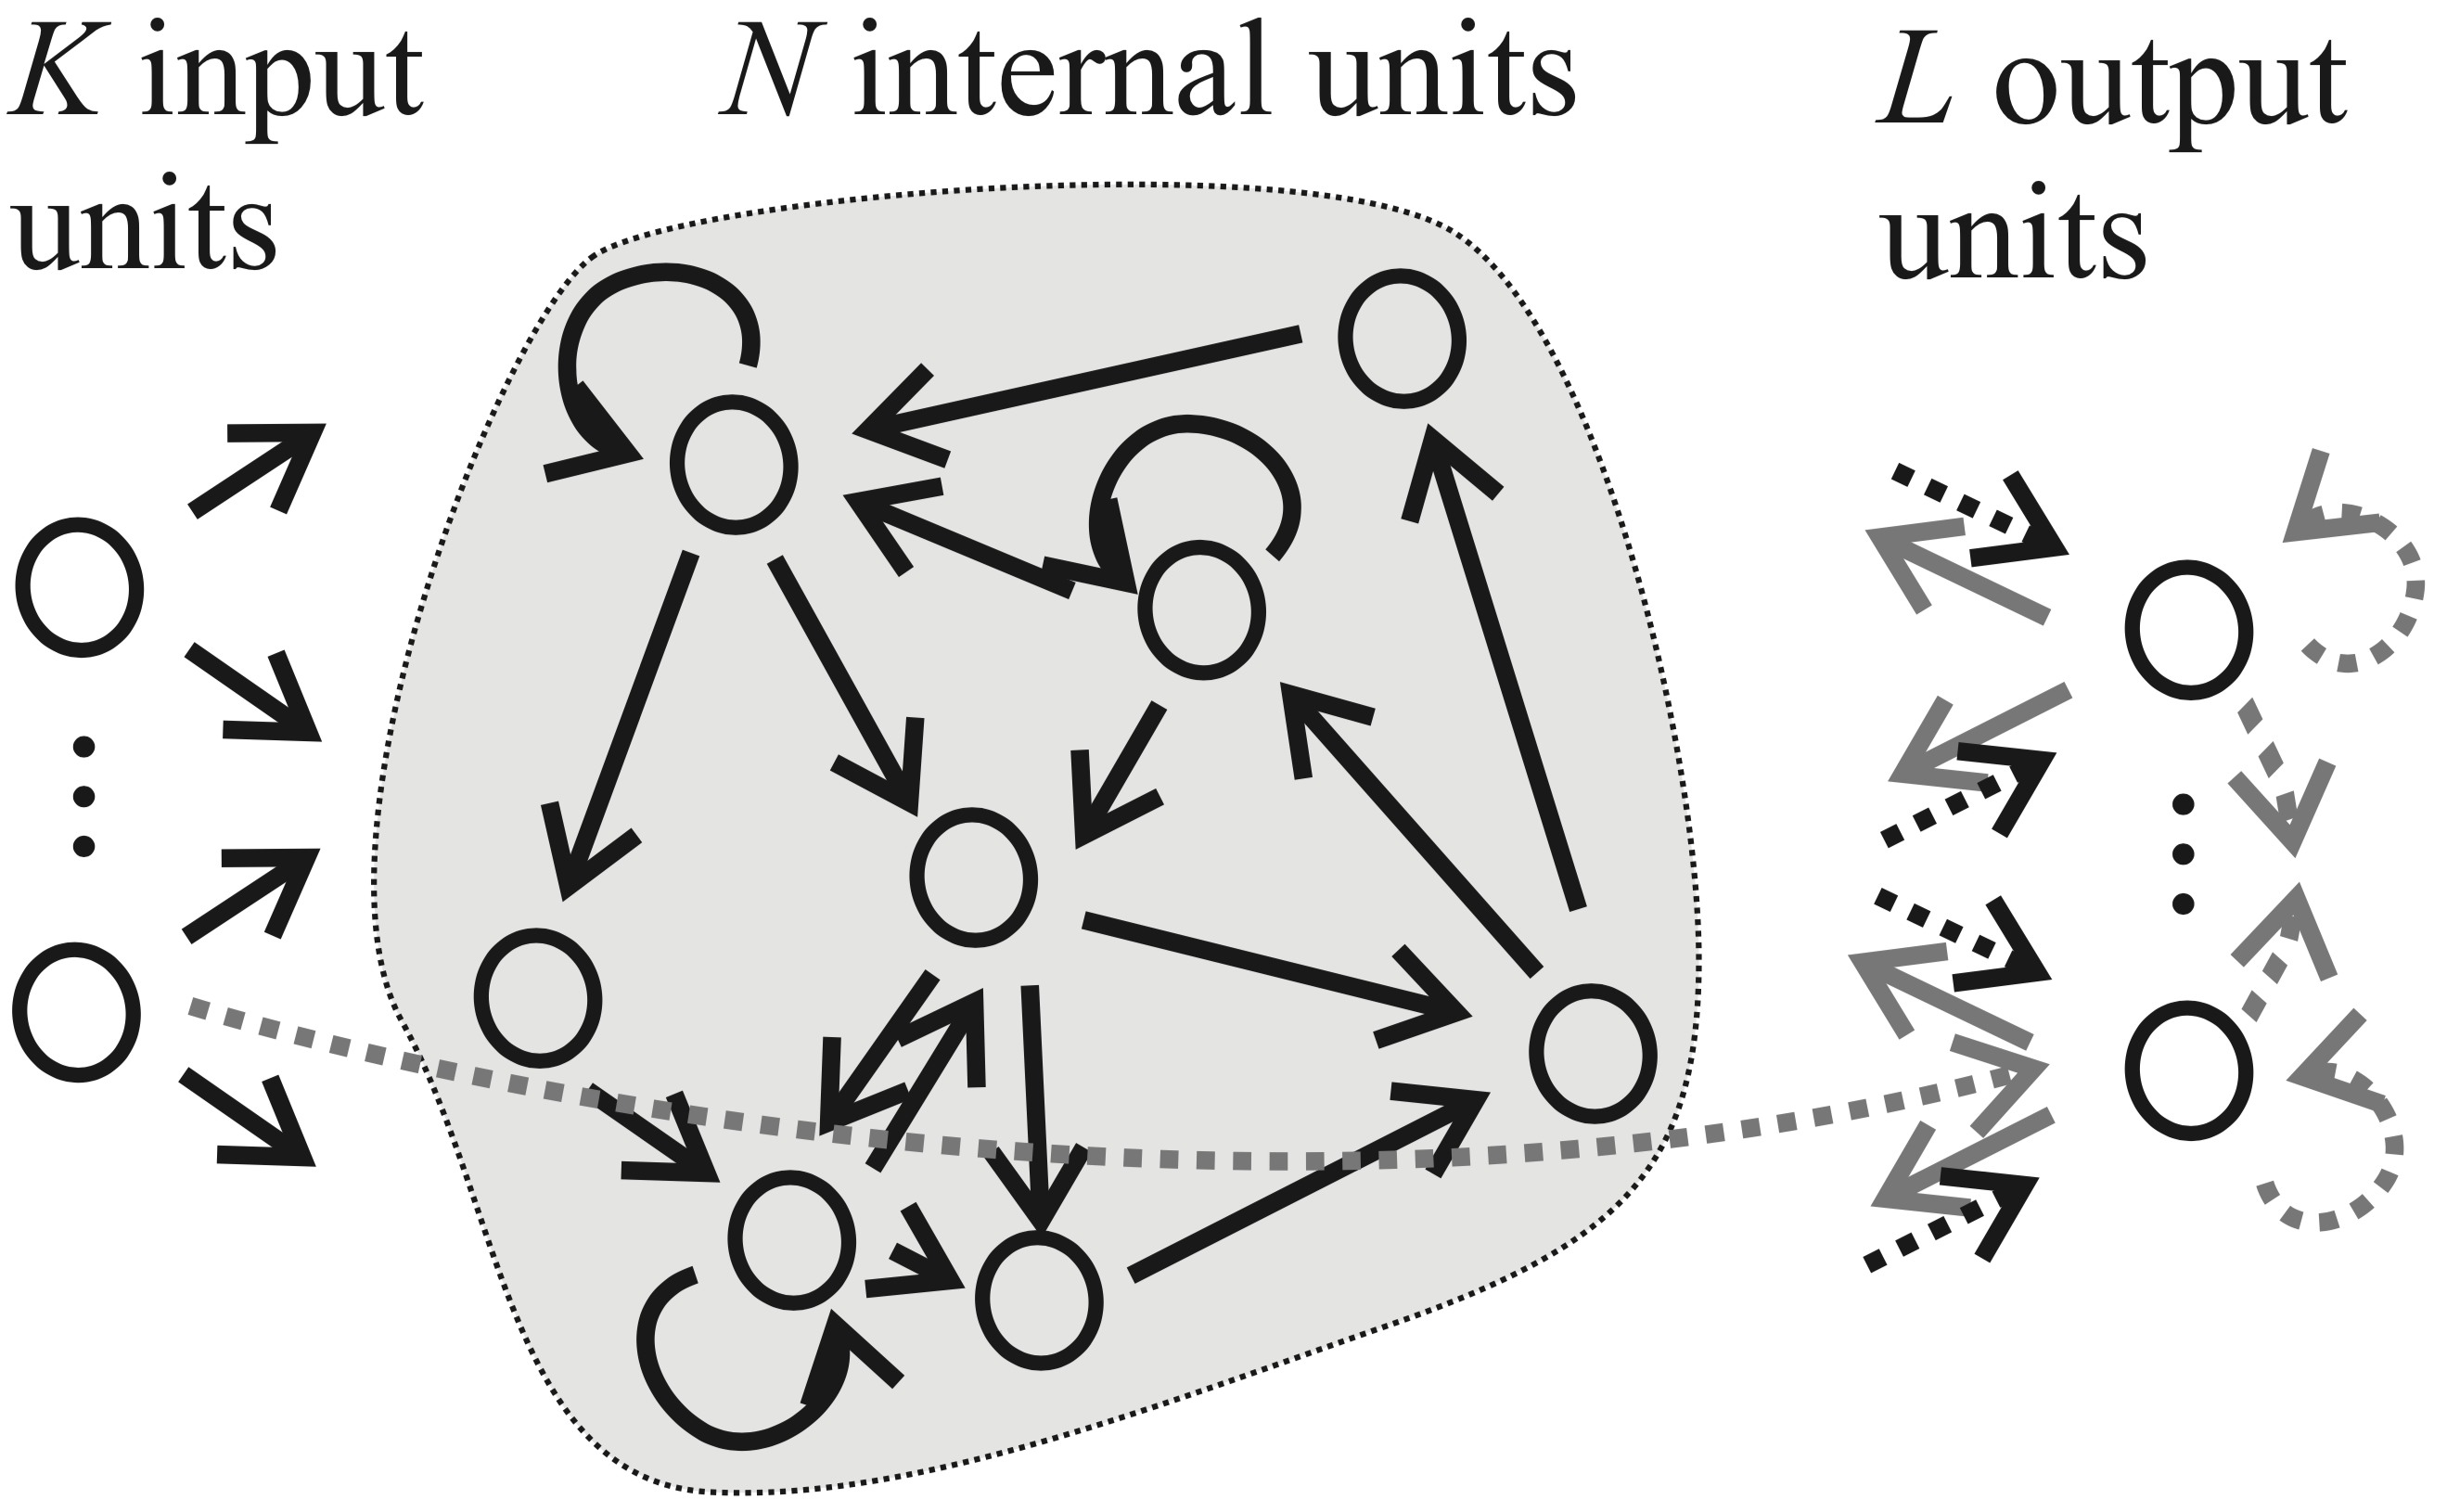
\includegraphics[scale=0.18]{reservoir.png}
     \caption{Source: \cite{jäger}.}
\end{figure}

\begin{itemize}
    \item $\text{Input to Reservoir with }\textbf{W}^{\text{in}}_{N\cross K}$
    \item $\text{Reservoir to Reservoir with }\textbf{W}_{N\cross N}$
    \item $\text{(Input + Reservoir + Output) to Output with }\textbf{W}^{\text{out}}_{L\cross (K+N+L)}$
    \item $\text{Output to Input with }\textbf{W}^{\text{back}}_{N\cross L}$
    
\end{itemize}

\begin{align}
    \textbf{x}(n+1) =  (1 - \alpha)\textbf x(n) + \alpha \cdot \textbf{f}(\textbf{W}^{\text{in}}\textbf u(n+1) + \textbf{W}\textbf{x}(n) + \textbf{W}^\text{back} y(n)), && \textbf{f}: \text{Reservoir activations}, \alpha: \text{Leaking rate}
\end{align}

\begin{align}
    \textbf{y}(n+1) = \textbf{f}^{\text{out}}(\textbf{W}^{\text{out}} \cdot concat(\textbf{u}(n+1),\textbf{x}(n+1) ,\textbf{y}(n))), && \textbf{f}^{\text{out}}: \text{Output activations}
\end{align}

\begin{definition}
\textbf{Standard compactness conditions}: \\
(i) input is drawn from a compact input space U \\
(ii) network states lie in a compact set A.
\end{definition}

\textit{\textbf{\textcolor{red}{\underline{From now on assume standard compactness conditions and a network without output feedback.}}}}

\begin{definition}
Iterator/state updater $T(\textbf x(n), \textbf y(n),\bar{\textbf u}^h) := \textbf x(n + h)
$, where $\bar{\textbf{u}}^h$ is the input sequence $\textbf u(n + 1), . . . , \textbf u(n + h)$
\end{definition}

\begin{definition}
Echo State Property (ESP) or Uniqueness of Solutions Property. Following statements are equivalent:

- Echo States $\textbf{x}$ are states uniquely determined by any $\bar{\textbf{u}}^{-\infty}$ and $T$ if network has no output feedback $\textbf{W}^{\text{back}}$.\\

- $\exists$ input echo functions $E = (e_1,...,e_N)$, where $e_i :\text{U}^{-N} \rightarrow R$, s.t. $\forall$ left-infinite input histories $..., u(n - 1), u(n) \in \text{U}^{- N}$ the current network state is $x(n) = E(..., u(n - 1), u(n))$.
\end{definition}

\begin{definition} Additional network properties

\begin{enumerate}[label=\Roman*.]
    \item Network is state contracting $\iff$ all reservoir states are similar on right-infinite inputs extending sufficiently far into the future.
    
    \item Network is state forgetting $\iff$ all reservoir states are similar on left-infinite inputs extending sufficiently far into the past.
    
    \item Network is state input forgetting $\iff \lim_{t\rightarrow \infty} \norm{H_U(\textbf{uz}_t^1) - H_U(\textbf{vz}_t^1)} = 0$, $H_U$ is functional associated to reservoir filter $U$, $\textbf{u,v}$ are semi-infinite sequences. $\textbf{z}_t^1$ is input at time t. So concatenating different inputs with the same input at infinite future yields indistinguishable output.
\end{enumerate}

\end{definition}

\begin{proposition}
Assume that T is continuous in state and input.
State contracting + state forgetting + input forgetting $\iff$ \text{ESP}. 
\end{proposition}

\begin{example}
$u(n) = sin(2\pi n/P)$, P: periodicity. Because of ESP the activations $x_i(n)$ are also periodic signals with the same period length P; but the network’s inhomogeneity induces conspicuous deviations from the input sinusoidal form. See paper for plots.

The 100-unit network used in the example was randomly connected; weights were set to values of 0, +0.4 and -0.4 with probabilities 0.95, 0.025, 0.025 respectively. This means a sparse connectivity of $5\%$. The value of 0.4 for non-null weights resulted from a global scaling such that $| \lambda_{max} | \approx 0.88 < 1$ (spectral radius) was obtained. How to scale is explained in the paper.
\end{example}

\begin{example}
(House of the Rising Sun) \underline{With output feedback with uniform random weigths}. $f^{out} = tanh$. A 400 unit sigmoid network was used. Internal connections were randomly as- signed values of 0, 0.4, -0.4 with probabilities 0.9875, 0.00625, 0.00625. This resulted in a weight matrix W with a sparse connectivity of 1.25\%. The maximal eigenvalue of W was $| \lambda_{max}| \approx 0.908$. The fact that spectral radius is close to 1 means that the network exhibits a long-lasting response to a unit impulse input. Generally, the closer spectral radius is to unity, the slower is the decay of the network’s response to an impulse input. A relatively long- lasting “echoing” of inputs in the internal network dynamics is a requisite for a sizable short-term memory performance of the network.

Problem: Reservoir states become periodic. Thus, minimization problem yields less equations in effect (linear dependence). Less than the dimension of $W^{out}$ making the system of equations underdetermined. This results in many possible perfect solutions. The 'naive' solution is unstable. Answer is to add uniform noise to \textbf y(n) which results in 'wobbling' states \textbf x(n).
\end{example}

\subsubsection{Multiple attractor learning}
TBP
\subsubsection{ESNs with leaky integrator neurons}
TBP. \href{https://quantumyilmaz.github.io/MTFS21/Examples/SimpleESN/large/SimpleESN_large.html}{\color{blue}See for Mackey-Glass example.}

\subsubsection{Key Takeaways}
\begin{itemize}
    \item Only the weights of connections leading to the output units are trained; all other connections remain un- changed. This makes it possible to employ any of the many available fast, constructive linear regression algorithms for the training. No special, iterative gradient-descent procedure is needed.
    
    \item We want that the eigenvalue of W with the largest absolute value (spectral radius) is smaller than 1. Otherwise network has an asymptotically unstable null state. This means no echo states for any input set U containing \textbf{0}. There should be no problem if the set does not contain \textbf{0}.
    \item We want sparse and random connections.
    
    \item On one hand waste of units (400 reservoir units in ESN can be done by say 20 LSTMs with gradient descent), on the other hand multi-tasking possibilities.
\end{itemize}

\subsection{ESNs are universal \cite{ortega,grigoryeva2018universal}}

\begin{align} \label{res_eq}
    \textbf{x}_t = F(\textbf{x}_{t-1},\textbf{z}_{t}) && F \text{: reservoir}, \textbf{x}_t \text{: reservoir state},\textbf{z}_t \text{: input signal},
\end{align}
\begin{align}
    \textbf{y}_t = h(\textbf{x}_t) && h \text{: readout},\textbf{y}_t \text{: output signal}
\end{align}

ESNs can be used as universal approximants in the context of discrete-time fading memory filters with uniformly bounded inputs defined on negative infinite times. 

A major breakthrough was the generalization to infinite time intervals carried out by Boyd and Chua in \cite{fadingmem}, who formulated a uniform approximation theorem using Volterra series for operators endowed with the so called \underline{fading memory property} on continuous time inputs.

\textbf{Fading memory property} says that inputs which are close in the recent past but not close in the remote past still yield close outputs in the present. Close here is in terms of peak deviation. From causal and TI filters one can go to the associated functional via the bijection map \cite{fadingmem}. Causal means inputs which were the same until now, yield same filter outputs now and their future values do not play a role. Then the condition to achieve FMP is a strengthened continuity of the functional (using weighted norm with a decaying weight sequence).

A discrete filter (not necessarily RC) with FMP can be approximated by SAS family (external approx.) and SAS can be approximated by ESNs (internal approx.).

ESNs are RCs with ESP. ESP holds when there is a state sequence \textbf{x} which solve the reservoir equation (\ref{res_eq}) for a given input sequence \textbf{z} and this state sequence is unique. 

ESP and FMP are difficult to check directly but there are other conditions that guarantee them. For example, contracting continuous reservoir maps with contraction constant less than 1 induce reservoir filters that automatically have the echo state and the fading memory properties. Similar but more restrictive yet easy to apply sufficient condition is to have spectral radius less than 1 and sigmoid activation function and states in $[-1,1]^N$.

\subsubsection{Notation and definitions}
\begin{itemize}
    \item $\textbf{Filters: } U:(D_n)^\mathbb{Z} \rightarrow \mathbb{R}^\mathbb{Z}$
    \item $\textbf{Functionals: } H:(D_n)^\mathbb{Z} \rightarrow \mathbb{R}$
    \item $\textbf{Causal: } z,w \in  (D_n)^\mathbb{Z}$ with $z_\tau=w_\tau, \forall \tau \leq t$ and $U(z)_t = U(w)_t \implies \text{Filter is causal}$
    \item $\textbf{Time Delay Operator: } U_\tau(z)_t = z_{t-\tau}$
    \item $\textbf{Time Invariant: } [U_\tau,U]=0$
    \item $\textbf{Filter determined by reservoir map: } U^F: (D_n)^\mathbb{Z} \rightarrow (D_N)^\mathbb{Z}$
    \item $\textbf{Reservoir Filter: } U^F_h(\textbf z)_t := h(U^F(\textbf z)_t)$, $h$:readout, F: Reservoir map
    
    \item $\textbf{Filter - Functional bijection: }$Given a time-invariant filter U, we can associate to it a functional $H_U(\textbf{z}):= U(\textbf{z}^e)_0$, where $\textbf{z}^e$ is an arbitrary extension of left-semi-infinite $\textbf{z}$ to infinity.
    Conversely, for any functional H we can define a time-invariant causal filter $U_H(\textbf{z})_t := H(\mathbb{P}_{\mathbb{Z}_{-}} \circ U_{-t})(\textbf{z}))$, where $U_{-t}$ is the $(-t)$-time delay operator and $\mathbb{P}_{\mathbb{Z}_{-}} : (D_n)^\mathbb{Z} \rightarrow (D_n)^{\mathbb{Z}_-}$ is the natural projection.
    
    \item $\textbf{Weighted Norm (of left semi-infinite sequences): } \norm{\textbf{z}}_w := \sup_{t \in \mathbb{Z}_{-}} \norm{\textbf{z}_t w_{-t}}$ , where $w_{n \in \mathbb{N}} \in (0,1]$ a monotonous zero sequence.
    
    \item   $l^\infty_w$ is the bounded sequence space with the weighted norm and is a Banach space.
    
    \item $\textbf{(Exponential) Fading Memory Property: } (w_n = \lambda^n, \lambda \in (0,1) ) H_U:((D_n)^{\mathbb{Z}_-},\norm{\cdot}_w) \rightarrow \mathbb{R}$. If $\exists w$ s.t. $|H_U(\textbf{z})-H_U(\textbf{s})| < \epsilon$ with  $\norm{\textbf{z}-\textbf{s}}_w = \sup_{t \in \mathbb{Z}} \{ \norm{(\textbf{z}_t-\textbf{s}_t)w_{-t}} \} < \delta(\epsilon)$. That means whenever there is a w s.t. $H_U$ is continuous.
    
\end{itemize}
\subsubsection{Key Takeaways}

\begin{itemize}
    \item Fading Memory Property implies input forgetting property.
    
    \item ESP and FMP imply uniqueness and continuity of solutions, respectively.
    
    \item ESP and FMP are difficult to check directly but there are other conditions that guarantee them such as local contractivity: If the reservoir map is a contraction and its contraction constant is less than 1. See also \cite{echo_index,Manjunath_2020}.

    \item Echo state property of the reservoir map $F$ implies causality and invariance of the filter $U^F$. 
    
    \item When a filter is causal and time-invariant it suffices to work with the restriction $U:(D_n)^{\mathbb{Z}_-} \rightarrow (D_n)^{\mathbb{Z}_-}$ instead of the original $U:(D_n)^\mathbb{Z} \rightarrow (D_n)^\mathbb{Z}$ since the former uniquely determines the latter.
    
    \item ESNs can be used as universal approximants in the context of discrete-time fading memory filters with uniformly bounded inputs defined on negative infinite times. Proven with internal (approximating unique RC filters) and external approximation (approximating some filter in general) properties.
    
\end{itemize}

\subsection{SigSAS \cite{teichmann}}

\subsubsection{Key Takeaways}

\begin{itemize}
    \item Network (aka filter) can be approximated by volterra series on uniformly bounded left infinite inputs. When this filter has additionally FMP the truncation error can be quantified.
    
    \item There is a state system SigSAS with ESP and FMP on uniformly bounded inputs. The state map inducing SigSAS and the continuous, time-invariant and causal associated filter have explicit forms. Any fading memory filter can be approximated up to monotonically decreasing rest term by this filter together with a trained linear readout. The quality of the approximation is not filter independent, as the decreasing sequence in the rest term depends on how fast the filter U “forgets” past inputs.
    
    \item The tensor space on which the SigSAS state filter is defined is high dimensional. This can be remedied by random projections in Johnson-Lindenstrauss Lemma. The random projections of the SigSAS system yield SAS systems with randomly generated coefficients in a poten- tially much smaller dimension which approximately pre- serve the good properties of the original SigSAS system. The loss in performance that one incurs because of the projection mechanism can be quantified using the Johnson-Lindenstrauss Lemma.
    
    
\end{itemize}

\subsection{Liquid State Machines (Maass) \cite{maass}}
Similar to ESNs but more biologically inspired. Uses spiking (integrate \& fire) neurons in the reservoir and readout and the connections from reservoir and the readout are trained via perceptron. The neurons fire (create a exponentially decaying spike train) when the successive sum of inputs pass some threshold value.

\section{HFT}

\subsection{Path Dependence \cite{pathdep} }
We said we do not want to concentrate on it for now.

\subsection{Hawkes Processes \cite{hawkes}}

\subsection{Reinforcement Learning \cite{reinforcement}}

\subsection{Irregular Time Intervals \cite{garch}}

\subsection{Mid-Price Strategies \cite{midprice}}

\subsection{Bars \cite{advances_in_ml}}

\begin{figure}[!htbp]
     \centering
     \textbf{Bar types}\par\medskip
     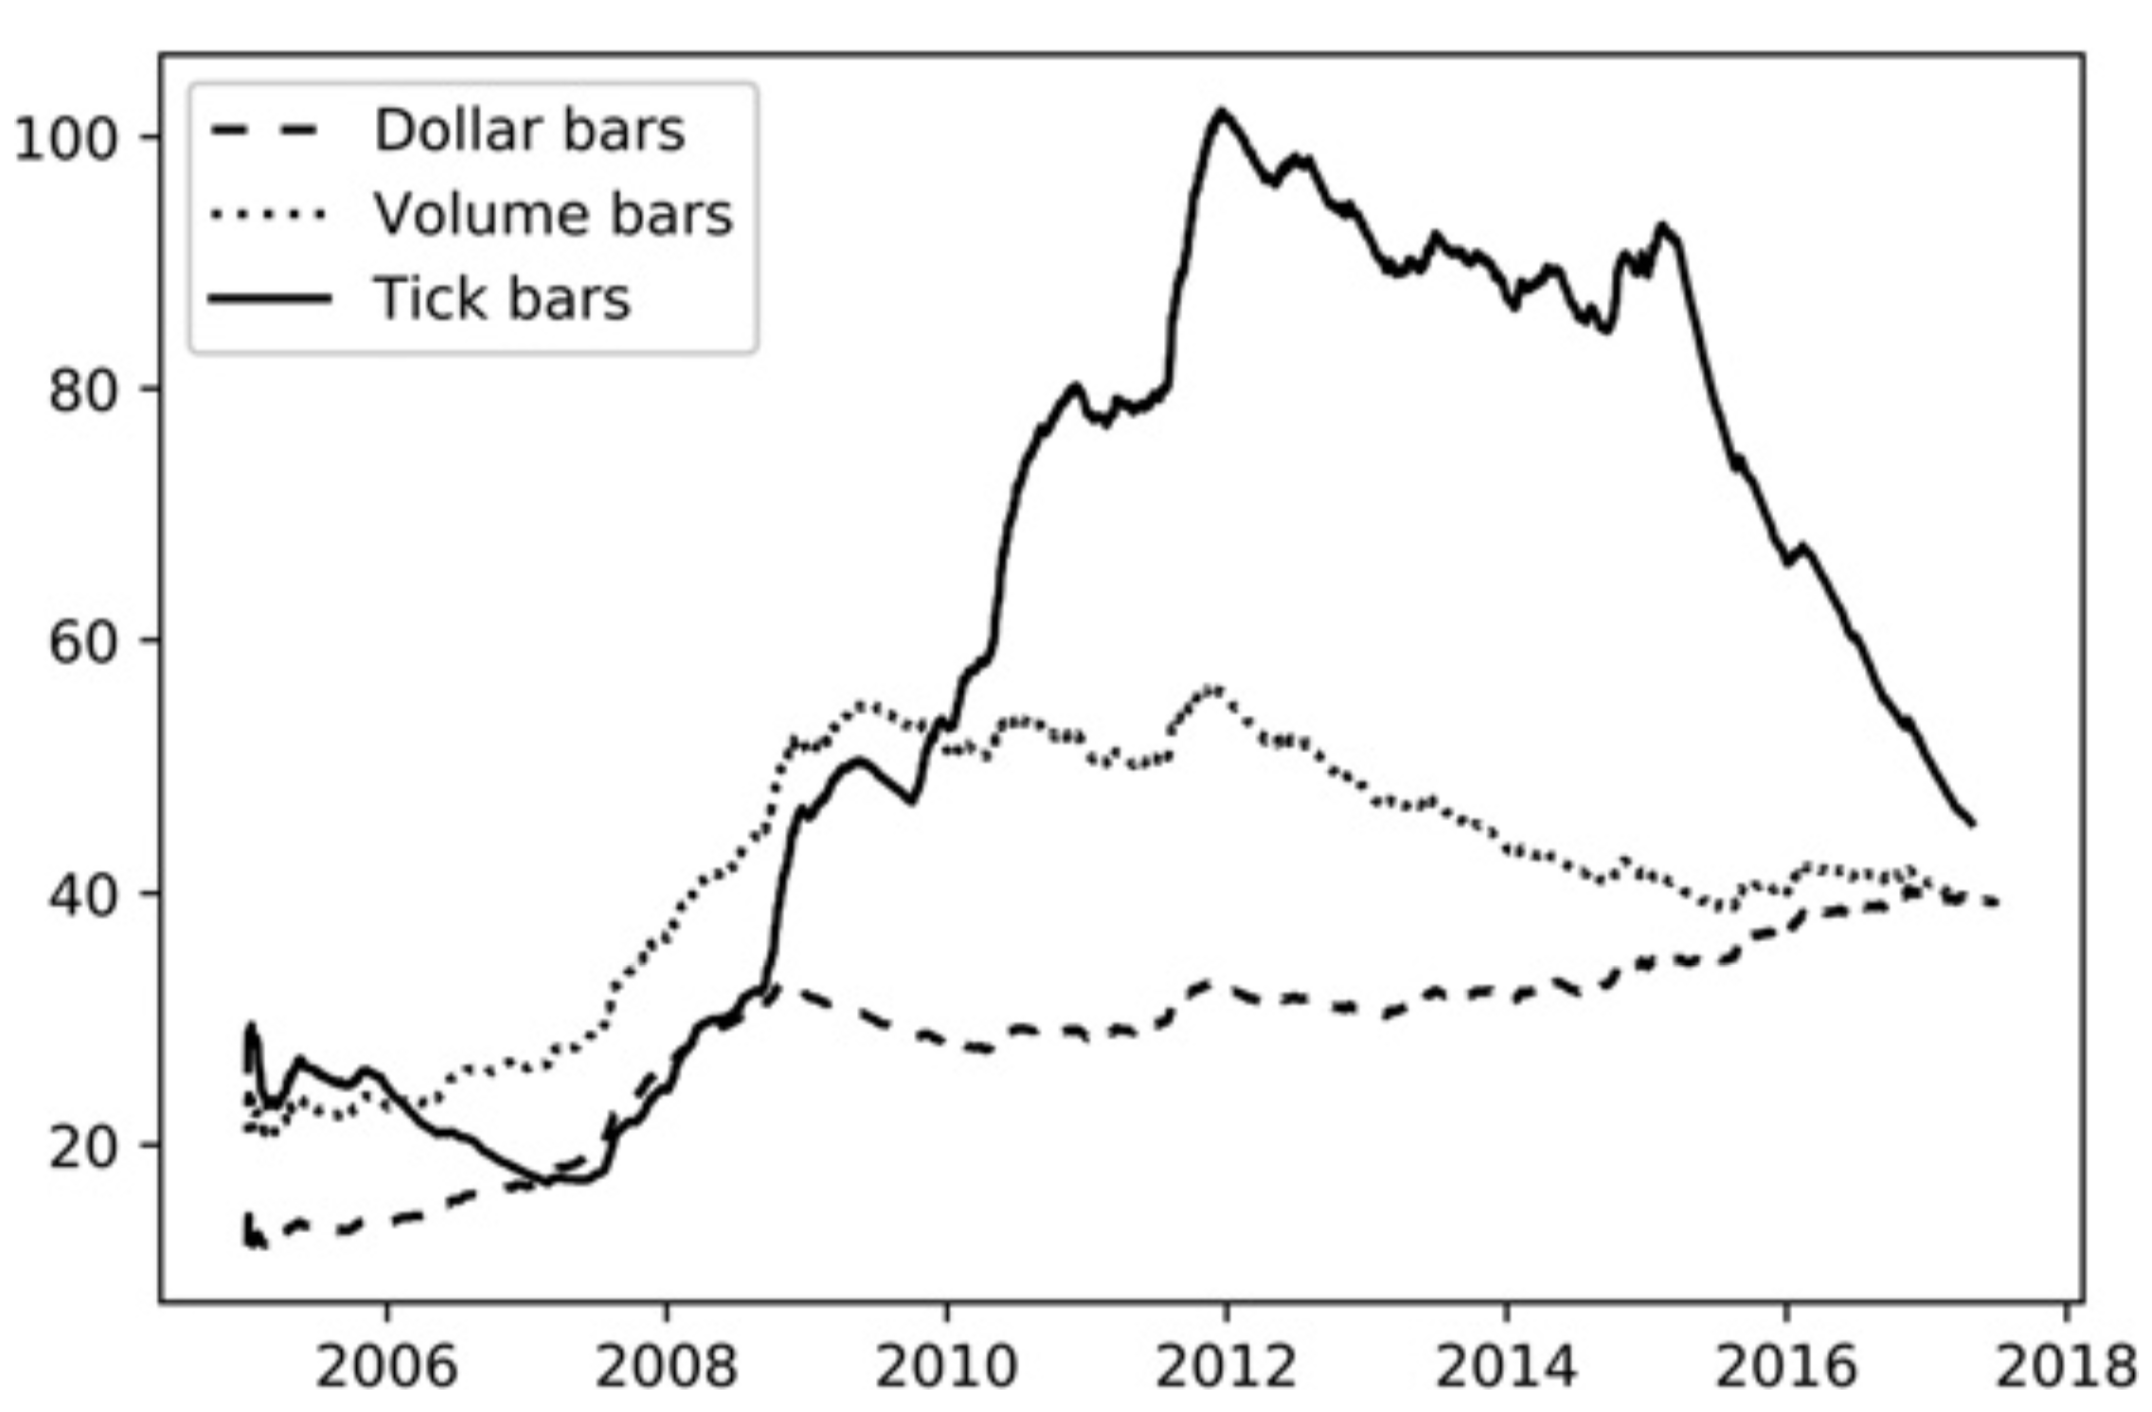
\includegraphics[scale=0.28]{bars.png}
     \caption{Source: \cite{advances_in_ml}}
\end{figure}

\subsubsection{Standard Bars}

\paragraph{Time Bars}
Bars are obtained over fixed time intervals.

\paragraph{Tick Bars}
Bars are extracted each time a predetermined number of transactions takes place. Tick bars allow for better inference than time bars.

\paragraph{Volume Bars}
Suppose that there is one order sitting on the offer, for a size of 10. If we buy 10 lots, our one order will be recorded as one tick. Volume bars circumvent that problem by sampling every time a predefined amount of the security’s units have been exchanged.

\paragraph{Dollar Bars}
The number of shares traded is a function of the actual value exchanged. Therefore, it makes sense sampling bars in terms of (dollar) value exchanged, rather than ticks or volume, especially in case of significant price fluctuations.

\subsubsection{Sampling}
\paragraph{CUSUM Filter}

\subsection{Triple Barrier Method \cite{advances_in_ml}}

\begin{figure}[!htbp]
     \centering
     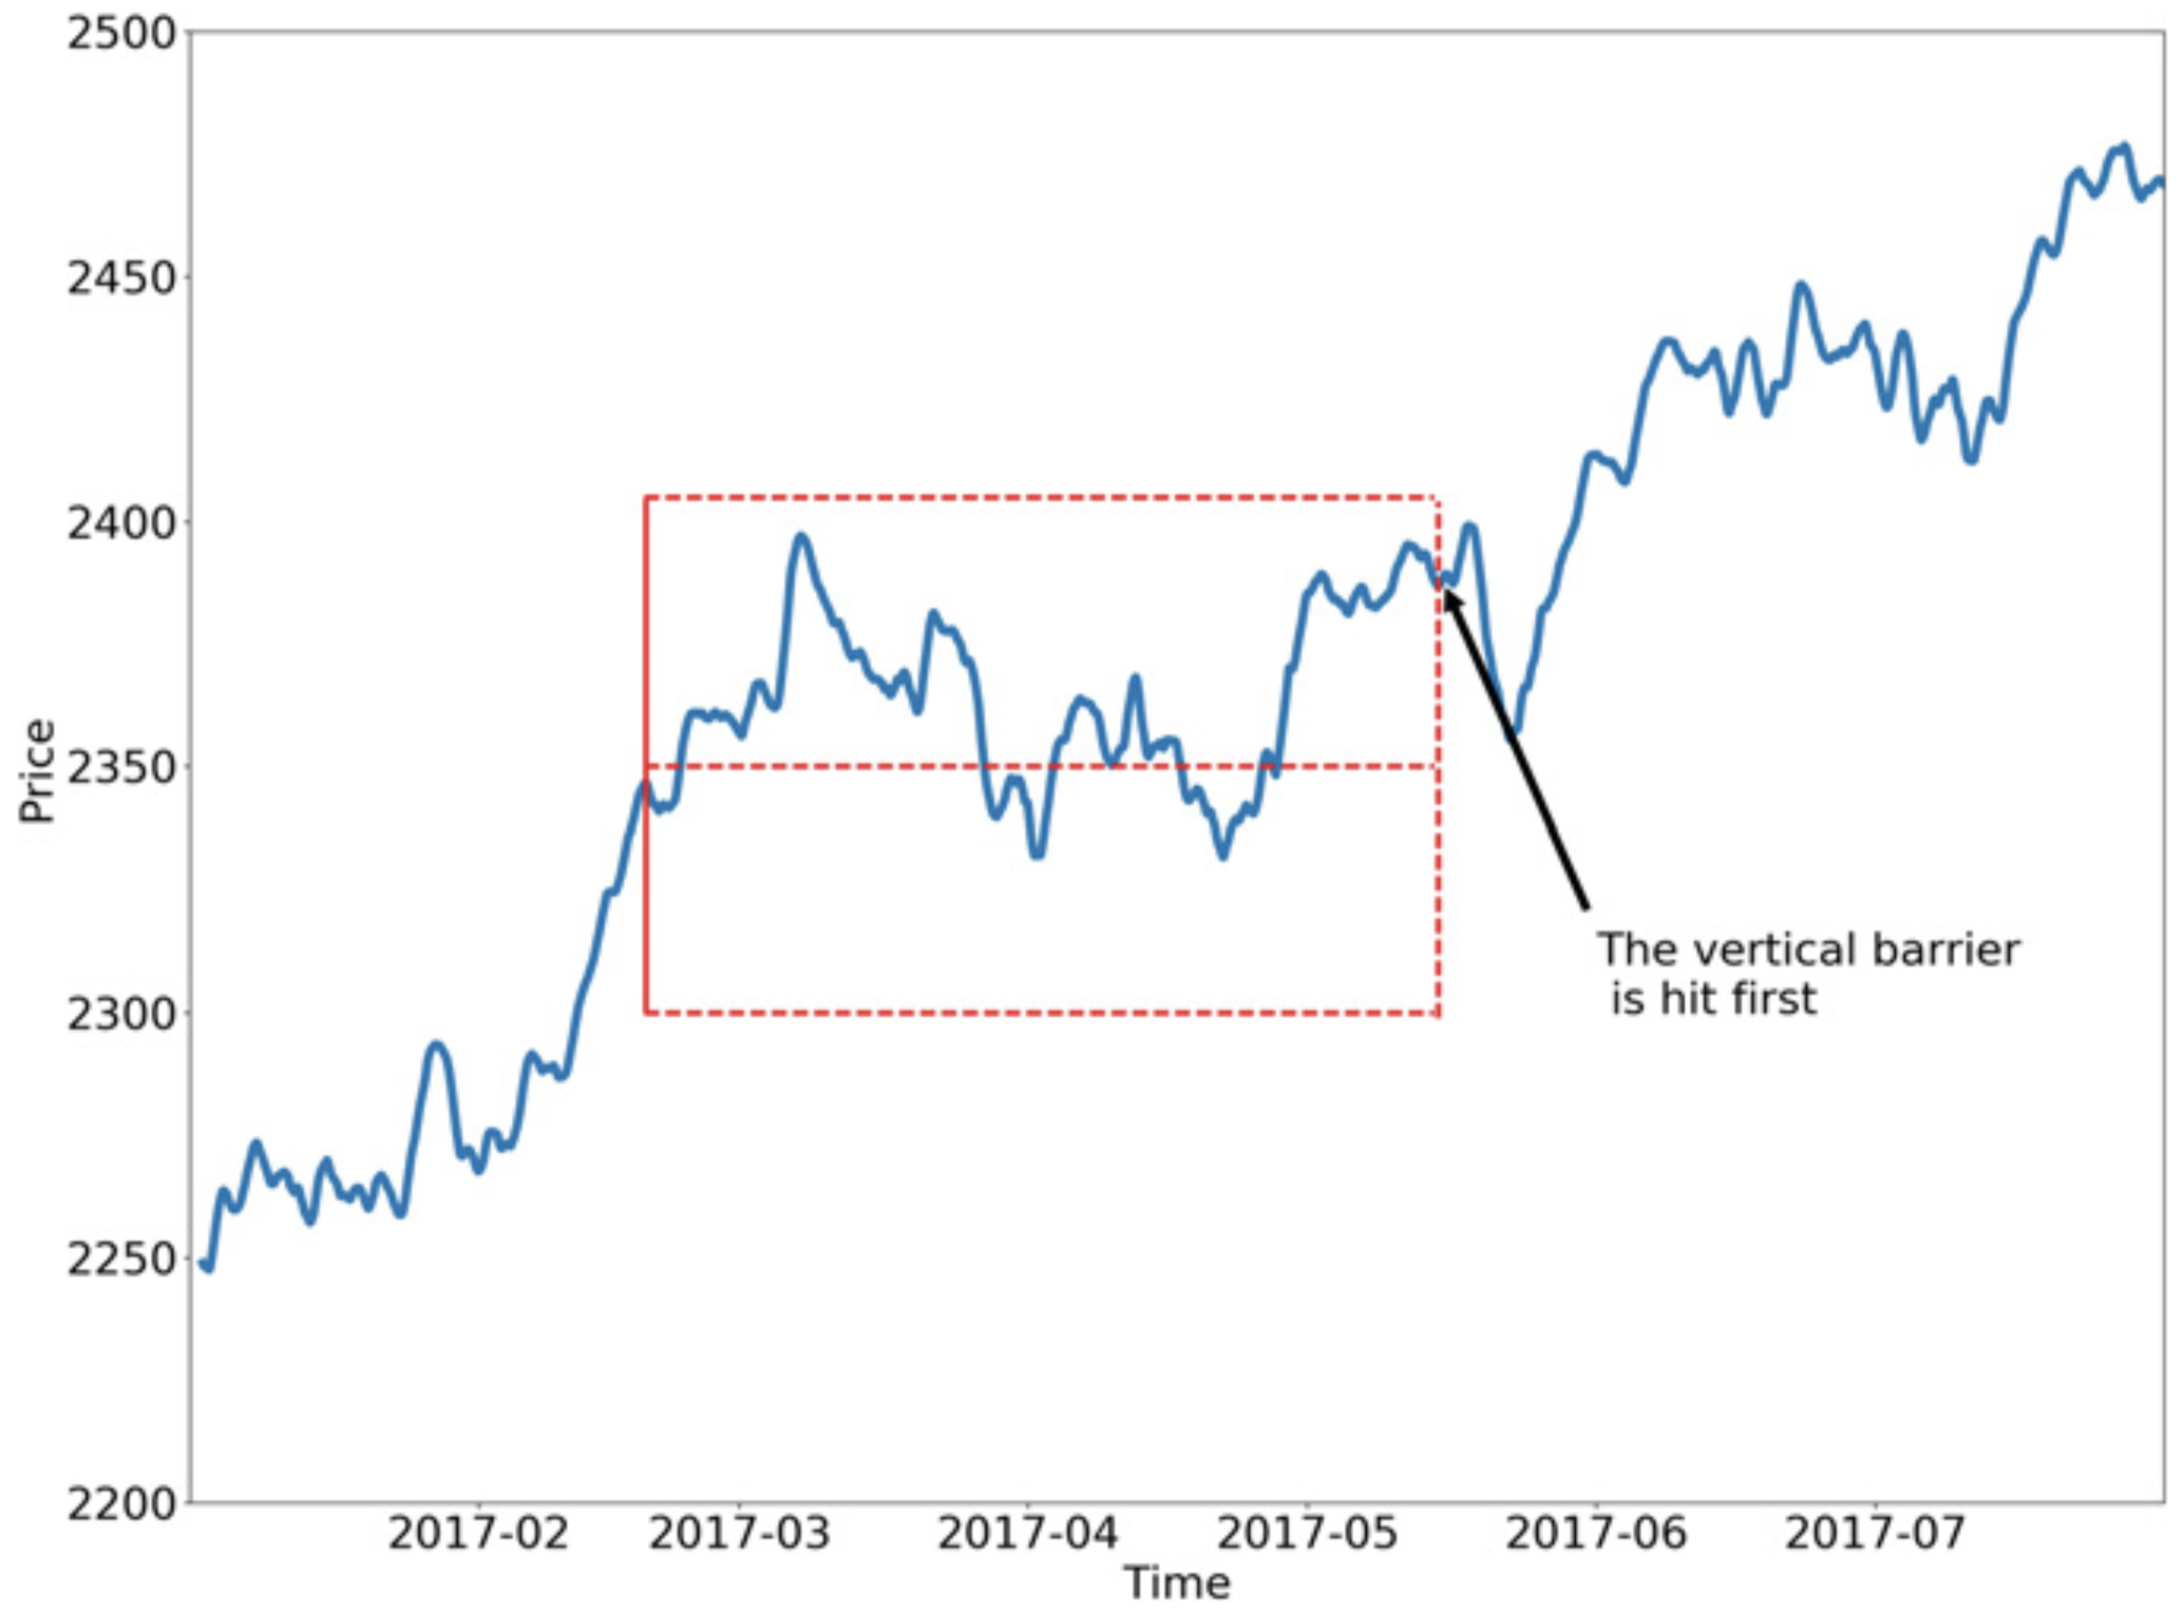
\includegraphics[scale=0.28]{3bar.png}
     \caption{Symmetrical barriers used for labelling the side of the trade. Source: \cite{advances_in_ml}}
\end{figure}

Triple Barrier method is used to learn the side of each trade. It is a path-dependent labelling strategy, which takes the problems of fixed-time horizon methods into account, such as autocorrelation, heteroscedasticity and volatility-independent thresholds, by imposing the following dynamic barrier rules:

\begin{enumerate}
    \item The upper barrier (profit-take) is hit first. Label = “1 (buy opportunity)”.
    
    \item The lower barrier (stop-loss) is hit first. Label = “-1 (sell opportunity)”.
    
    \item The vertical barrier (expiration) is hit first. Label = sign of the return or a 0.
\end{enumerate}

The idea is to teach the these labels to a machine learning algorithm in a supervised setting, where \textbf{Exponentially Weighted Standard Deviations (EWSD)} (\ref{EWSD}) computed from returns inside a predetermined time frame prior to each barrier are used to determine the horizontal barrier widths. A front (vertical) barrier is also placed acting as an expiration limit. If it is hit first and the corresponding label is chosen as 0, then it indicates that there is no trading opportunity.


\begin{equation} \label{EWSD}
    \text{EWSD}_{t_k} = \sqrt{ b_k \cdot \frac{\sum^k_{i=0} w_i (x_{t_{k-i}} - \text{EWMA}_{t_k})^2}{\sum^k_{i=0} w_i} }
\end{equation}

\begin{itemize}
    \item $\alpha: \text{the smoothing factor}$
    \item $w_i = (1 - \alpha)^i$
    \item ${t_k} \in \{ t_n |t_n - t_{n-1} = \text{predetermined time length } \forall n \in \mathbb{N}^{+},t_0: \text{first registered time in dataset} \}$
    \item $x_{t_k}: \text{return}$ with $x_{t_k} = price_{t_k}/price_{t_{k-1}} - 1$
    \item $b:\text{bias}$ with $b_k = \frac{(\sum^k_{i=0} w_i)^2}{(\sum^k_{i=0} w_i)^2 - \sum^k_{i=0} w_i^2}$
    \item $\text{Exponentially Weighted Moving Average EWMA}_{t_k} = \frac{\sum^k_{i=0} w_i x_{t_{k-i}}}{\sum^k_{i=0} w_i}$
\end{itemize}

After the data is divided into windows with predetermined time frames and triple barrier labels are attached to these, a model is given previous prices as input and trained to learn the labels. 

In our case, the data is divided into 30 minute windows. Looking at prior 30 minutes a standard deviation (\ref{EWSD}) is calculated. Using this, the horizontal barriers are placed. A vertical barrier at 30 minutes ahead is placed. This is done for each bar in the Limit Order Book (LOB) starting from 30 minutes after the first bar in LOB. The model is given the previous 30 minutes' prices as input, including the price at the minute, where it is expected to yield a label, i.e. forecast the correct position: long, short or do nothing. So each input consists of 31 prices. The windows for which exactly 31 bars are not available in the LOB are removed during data preparation as well as time bars before 10:00 AM and after 18:00 PM, belonging to single price auctions in Borsa Istanbul.

\subsubsection{Meta-Labelling}\label{sec::meta}
A secondary model could be used to assess the confidence in the labels from the primary model described previously. In our case, binary confidences are calculated, i.e. for each prediction from the primary model a label $\in \{0,1 \}$ is given by the secondary model. The continuous case $(0,1)$ will be explored soon. 

The goal here is to reduce false positives which could be costly in some trades, at the expense of true positives, where true positive rate (TPR) will be reduced and the precision will be increased. It takes the predictions of the primary model as input and the correct labels are given as output. In our case this is done by training reservoirs. The results are shown in Figure \ref{fig:triple_label_scores}.

\begin{figure}[!htbp]
  \centering
  \subfloat[a][Scores of reservoirs trained with different activation functions.]{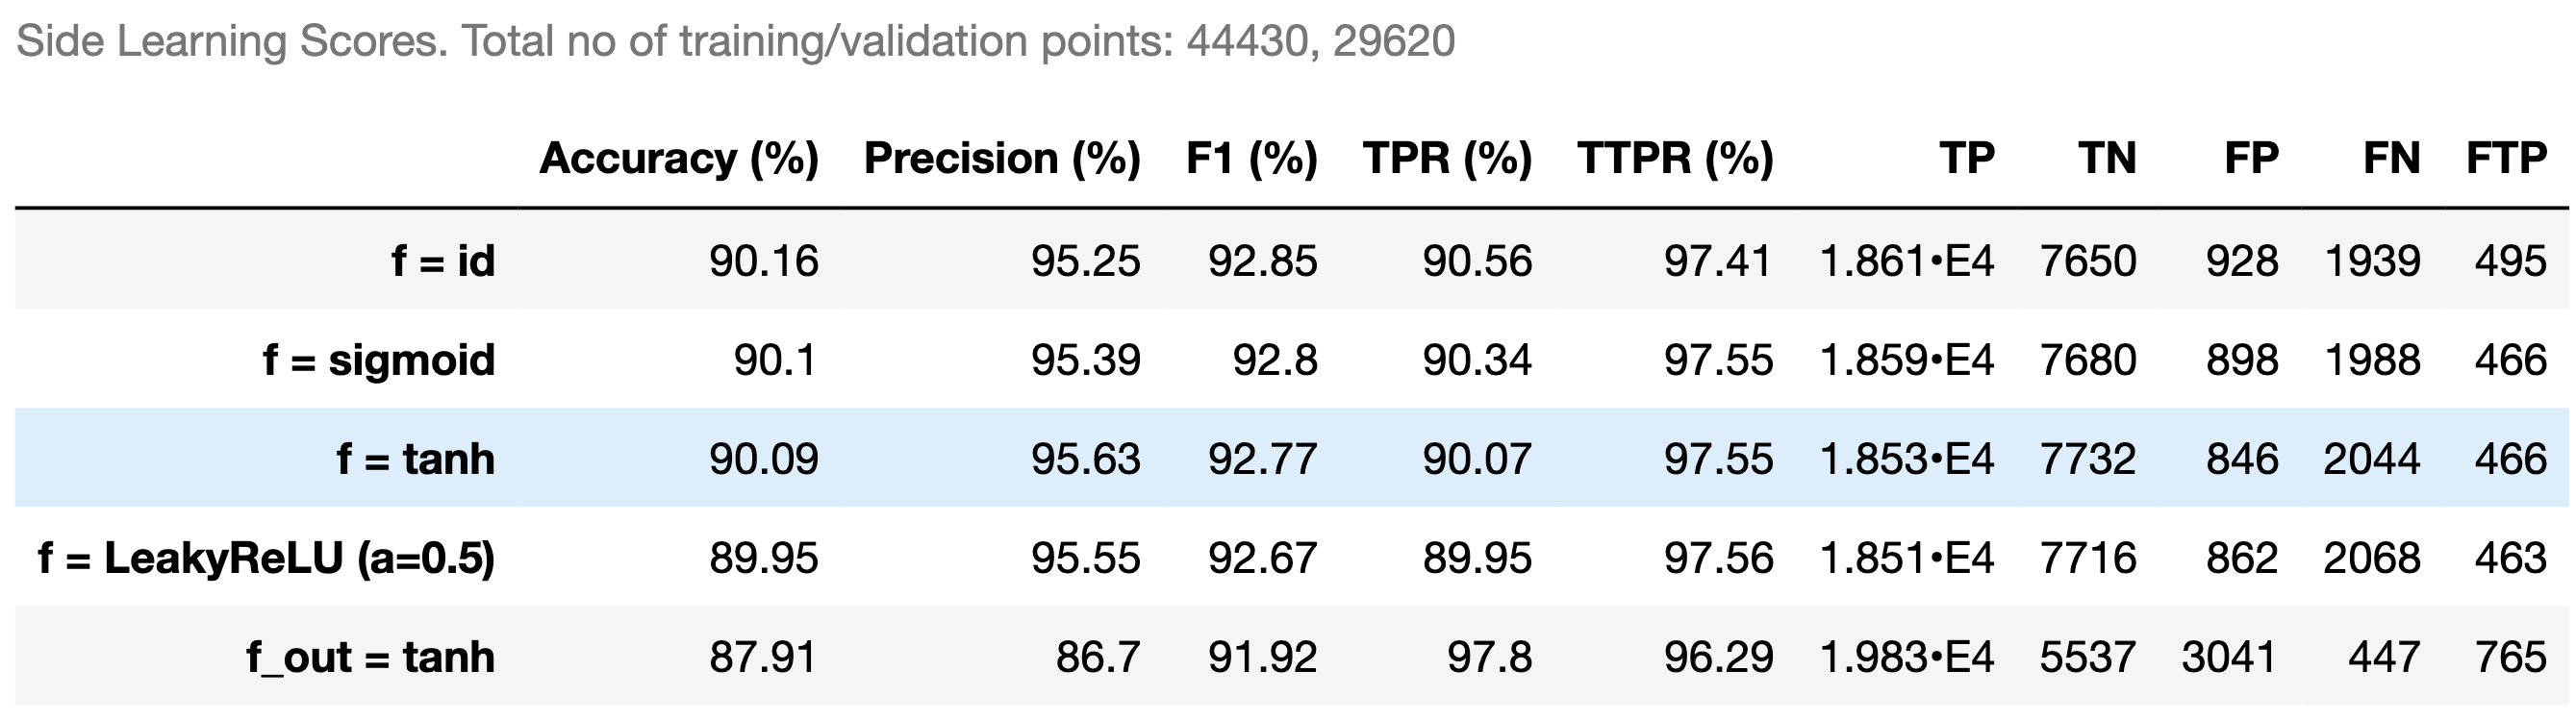
\includegraphics[scale=0.3]{label_scores.png} \label{fig:label_scores}} \\
  \subfloat[b][Scores of meta-reservoirs trained with different activation functions on labels of different reservoirs.]{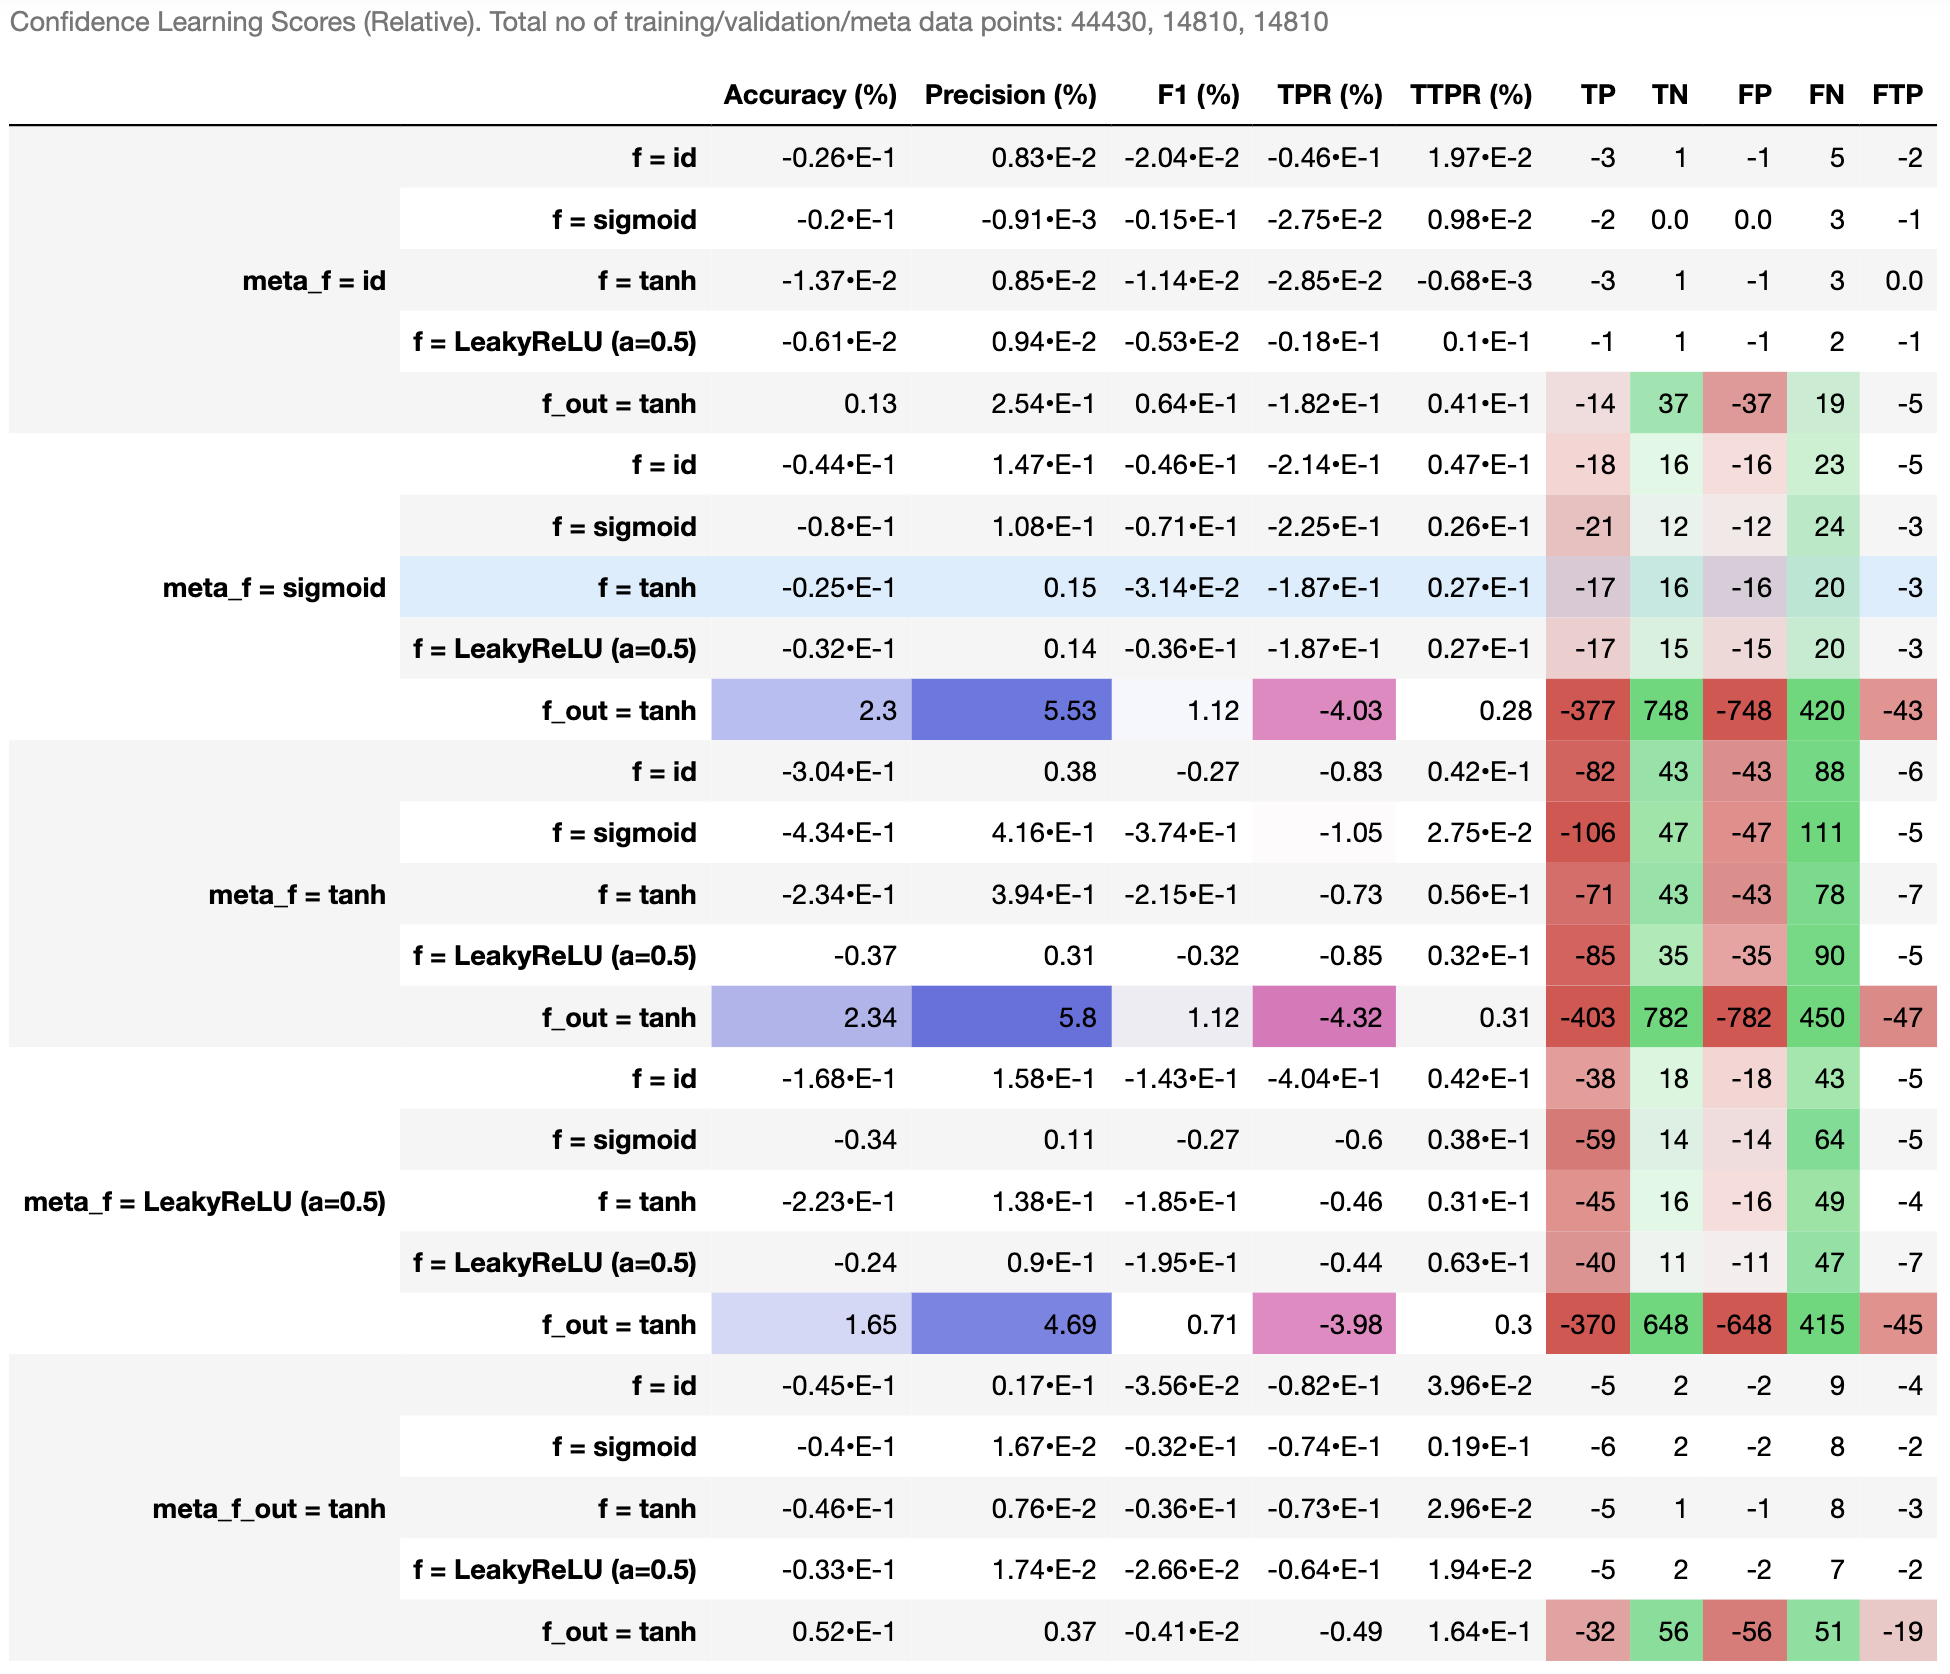
\includegraphics[scale=0.4]{meta_scores.png} \label{fig:meta_scores}}
  \caption{Triple Barrier label scores. TTPR is given by TP/(TP+FTP) and FTP is the number of correct identification of trading opportunities with incorrect side.} \label{fig:triple_label_scores}
\end{figure}

\subsubsection{Barrier Widths}\label{sec::barr_widths}
Learning the side of the trade, we needed to be fair to both possible positions (long and short) and for that we have utilized symmetrical horizontal barriers. Once a model knows the correct side of a trade, putting actual profit taking and stop-loss barriers is the next step, which do not need to be symmetrical. For this purpose a model is trained to forecast the maximum available return inside a given window as well as the minimum return observed before hitting this maximum return.

In our case the model takes previous 31 prices including the price at the minute of position taking, the return of the previous 30 minute interval (see $x_{t_k}$ in (\ref{EWSD})), EWSD and EWMA as input of length 34.

\subsubsection{Application}\label{sec::application}
Once (meta-labelled) side predictions, profit taking targets and stop-loss thresholds are available, a trading experiment can bu run.

The data is divided into three subsets: 
\begin{enumerate*}
    \item Training
    \item Validation
    \item Meta
\end{enumerate*}.
A primary model is trained on the blue part in Figure \ref{fig::data_split} to learn the labels of sides. These labels are filtered through a meta-labelling model described in \ref{sec::meta}.
This meta-label model is trained on the orange part in Figure \ref{fig::data_split}, i.e. on the first half of the validation of the primary model. Lastly another model is taught the barrier widths described in \ref{sec::barr_widths} with a training domain of blue+orange in Figure \ref{fig::data_split}. Its validation domain is the same as meta-labelling model's validation domain, the green part. This is where the experiment is run.

Each minute in the green domain, using the resulting predictions from previously described stages, we look at 30 minute windows. If the profit taking barrier is exceeded during this period given that the stop-loss barrier is not hit prior to that, the model executes the trade at that minute. If the stop-loss barrier is hit first, then the position is ended there. If none of the non-symmetrical barriers are hit, the position is ended at the vertical barrier, i.e. after 30 minutes and the positive (negative) return at that point is added (subtracted) from the wallet. The bet size is given by the total capital divided by the price of the asset at the time of the position. 

Currently, the experiment is run on bid prices. A more realistic case where both bid and ask prices are used for buying and selling the asset will be investigated. Furthermore, a scenario where the algorithm is only allowed to invest $\frac{\text{available volumes} \cdot \text{bid/ask price}}{100}$ TL will also be investigated. The current setting yields 223.5 B with an initial capital of 100 within a trading period of approx. 51 days.
\clearpage

\begin{figure}[!htbp]
     \centering
     \textbf{Data Subsets}\par\medskip
     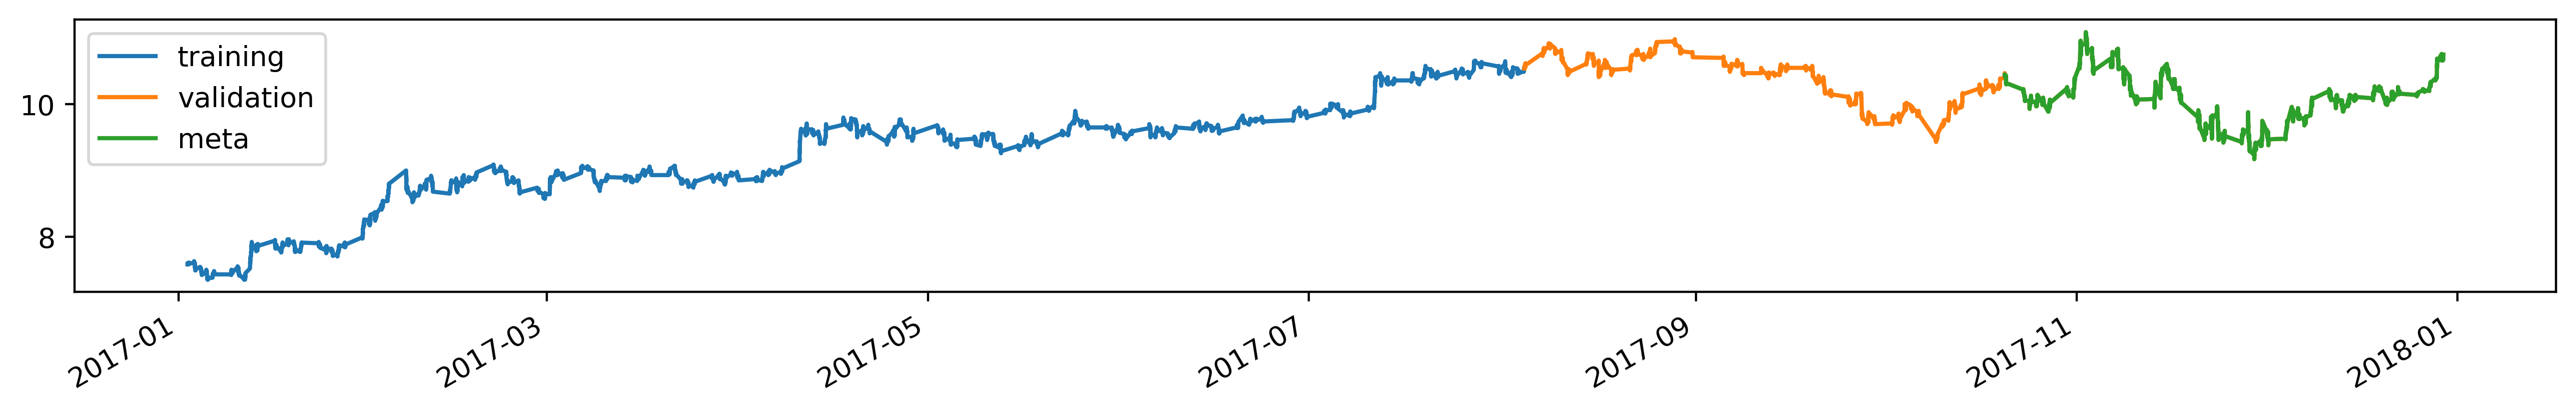
\includegraphics[scale=0.48]{data_split.png}
     \caption{Ratios of subsets (from left to right) to total length is 3:1:1}
     \label{fig::data_split}
\end{figure}

\begin{center}
    \underline{Summary of Experiment}
    \begin{itemize}
        \item Initial capital: 100
        \item Tot. Returns: $2.235 \cdot 10^{11}$
        \item No of loss-making trades: 3126
        \item No of profitable trades: 4984
        \item Gains: $2.588 \cdot 10^{11}$
        \item Losses: $3.533 \cdot 10^{10}$
        \item Time frame: 51 days 2 hours 3 minutes
    \end{itemize}
\end{center}

\begin{figure}[!htbp]
  \centering
  \subfloat[a][Total capital throughout the trading session]{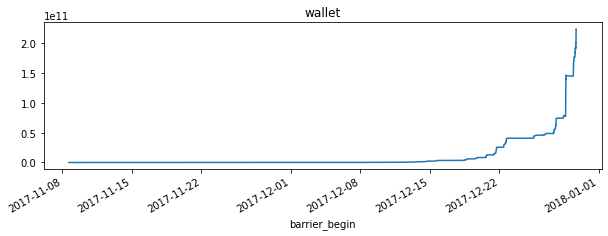
\includegraphics[scale=0.4]{wallet.png} \label{fig:wallet}} \\
  \subfloat[b][Profits and Losses throughout the trading session]{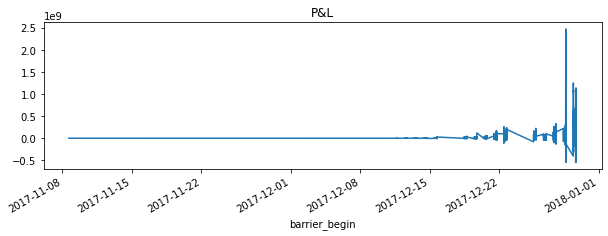
\includegraphics[scale=0.4]{p_n_l.png} \label{fig:p_n_l}}
  \subfloat[c][Bet sizes throughout the trading session]{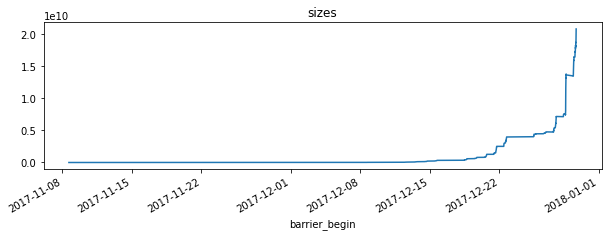
\includegraphics[scale=0.4]{sizes.png} \label{fig:sizes}}
  \caption{Plots from the experiment described in \ref{sec::application}} \label{fig:AB}
\end{figure}




\clearpage
\printbibliography
\end{document}